%!TeX root=../main.tex

% -- Weight solutions vs. Architectures solutions
Creating network architectures which encode solutions is a fundamentally different problem than that addressed by neural architecture search (NAS). 
% [encode biases toward solutions, which encode solutions] <- awk.
The goal of NAS techniques is to produce architectures which, once trained, outperform those designed by humans. 
%
It is never claimed that the solution is innate to the structure of the network. 
% 
Networks created by NAS are exceedingly `trainable' -- but no one supposes these networks will solve the task without training the weights. 
% [exceedingly] <-- better syn?
The weights \textit{are} the solution; the found architectures merely a better substrate for the weights to inhabit.

To produce architectures that themselves encode solutions, the importance of weights must be minimized. 
%
Rather than judging networks by their performance with optimal weight values, we can instead measure their performance when their weight values are drawn from a random distribution.
%
Replacing weight training with weight sampling ensures that performance is a product of the network topology alone.
%
Unfortunately, due to the high dimensionality, reliable sampling of the weight space is infeasible for all but the simplest of networks.
% [reliable] <-- better syn?

% -- Weight-sharing allows sampling of large networks
Though the curse of dimensionality prevents us from efficiently sampling high dimensional weight spaces,  
%Though sampling of a high-dimensional weight space is not practical,
by enforcing weight-sharing on \textit{all} weights, the number of weight values is reduced to one.
%
Systematically sampling a single weight value is straight-forward and efficient, enabling us to approximate network performance in only a handful of trials.  
%
This approximation can then be used to drive the search for ever better architectures. 


% Summarize Algorithm:
The search for these weight agnostic neural networks (WANNs) can be summarized as follows (See Figure \ref{fig:overview} for an overview): 
%
\textbf{(1)} An initial population of minimal neural network topologies is created, 
%
\textbf{(2)} each network is evaluated over multiple rollouts, with a different shared weight value assigned at each rollout, 
%
\textbf{(3)} networks are ranked according to their performance \textit{and} complexity, and 
%
\textbf{(4)} a new population is created by varying the highest ranked network topologies, chosen probabilistically through tournament selection~\cite{tournamentSelection}. 
%
The algorithm then repeats from \textbf{(2)}, yielding weight agnostic topologies of gradually increasing complexity that perform better over successive generations.

%!TeX root=../main.tex

\begin{figure}[th!]
\vskip -0.05in % useful knobs to optimize layout
    \centering        
    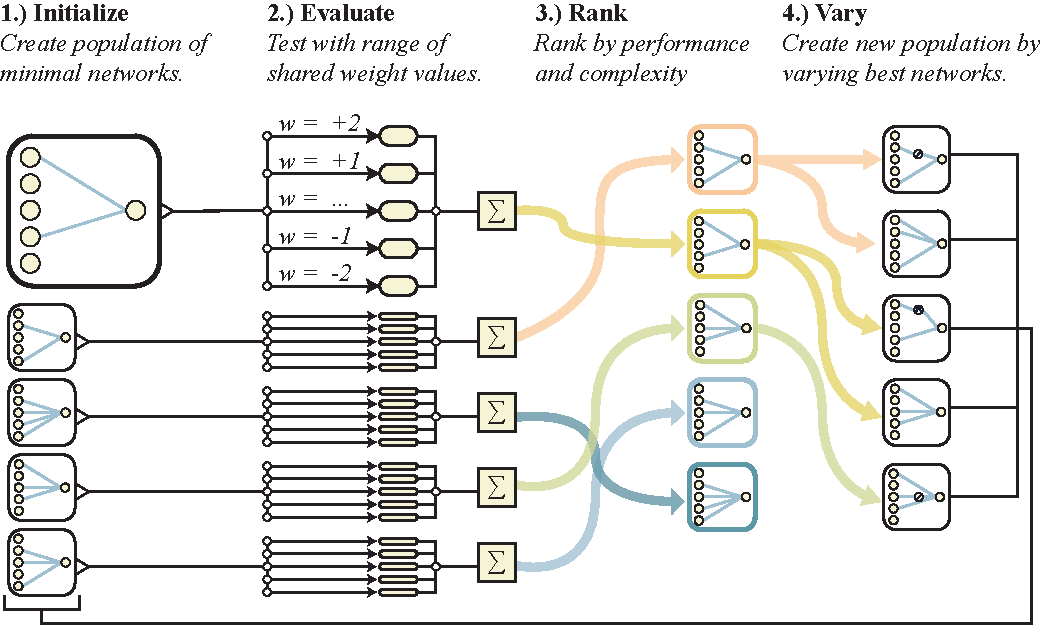
\includegraphics[width=1\textwidth]{img/wann.pdf}   
\vskip -0.05in % useful knobs to optimize layout
    \caption      
    {     
        \textit{Overview of Weight Agnostic Neural Network Search}
        \newline
        Weight Agnostic Neural Network Search avoids weight training while exploring the space of neural network topologies by sampling a single shared weight at each rollout. 
        %
        Networks are evaluated over several rollouts. At each rollout a value for the single shared weight is assigned and the cumulative reward over the trial is recorded. 
        %
        The population of networks is then ranked according to their performance and complexity. 
        %
        The highest ranking networks are then chosen probabilistically and varied randomly to form a new population, and the process repeats.
    }         
    \label{fig:overview}
\vskip -0.15in % useful knobs to optimize layout
\end{figure}


